\documentclass{standalone}

\begin{document}

\subsection[Super Resolution Models]{Super Resolution Models}\label{SR:wdsr}

\begin{center}
\begin{figure}[htbp]
\centering
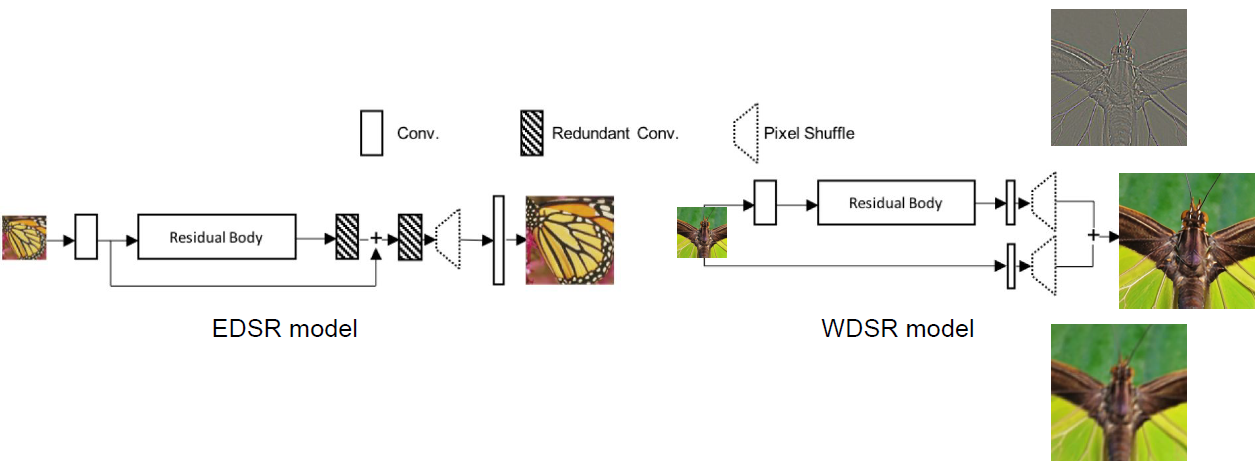
\includegraphics[width=0.85\textwidth]{SR_models.png}
\caption{Super Resolution models analyzed in this work.
\textbf{(left)} EDSR model.
The model is a modified version of the ResNet architecture designed for SISR applications.
The architecture is made by a sequential CNN framework, which processes the input image.
The EDSR has more than $43$ million of parameters in total.
\textbf{(right)} WDSR model.
The model is the updated version of the EDSR one.
The model optimizes its numerical efficiency using a different approach in the analysis of low- and high-frequency components in the input image.
The WDSR has slight more than $3.5$ million of parameters, less than $10$\% of the EDSR model.
}
\label{fig:sr_models}
\end{figure}
\end{center}

There were different kinds of models proposed for image Super Resolution purposes, but in this work we focused only on two of them.
Both are based on deep learning Neural Network models and they became famous in the research community since they both won the last NTIRE editions, 2017 and 2018 respectively.

\begin{table}[htbp]
\centering
\begin{tabular}{lccc}
\hline \rowcolor{darkgrayrow}
                         &  Channels     & Filter     & Number of    \\
\rowcolor{darkgrayrow}
Layer                    & input/output  & dimensions & Parameters   \\
\hline
Conv. input              & 3/256      & $3\times3$   & 6912    \\
Conv. (residual block)   & 256/256    & $3\times3$   & 589824  \\
conv. (pre-shuffle)      & 256/256    & $3\times3$   & 589824  \\
Conv. (upsample block)   & 256/1024   & $3\times3$   & 2359296 \\
Conv. output             & 256/3      & $3\times3$   & 6912    \\
\hline
\end{tabular}
\caption{EDSR model scheme summary.
We highlight the number of parameters of each macro-block.
The total number of parameters of this model is given by the sum of the values in the last column (more than 3 million of parameters).
}
\label{tab:edsr}
\end{table}

The first model is called EDSR (\emph{Enhanced Deep Super Resolution}) and was firstly proposed at the NTIRE challenge in 2017~\cite{Agustsson_2017_CVPR_Workshops}.
The EDSR model structure could be broadly summarized as an updated version of the SRResNet model, which is already a modified version of the classical ResNet (standard CNN based on multiple residual blocks).
The major updates concern a series of optimizations to improve the training speed and the quality of the output image.
In particular, the batch normalization steps are removed to improve the speed of the algorithm: it was proved that in low-level vision tasks as the super resolution one, i.e without complex evaluations as object detection, a wide and dynamic range of outputs can be useful~\cite{edsr}.
A scheme of the EDSR architecture is shown in Fig.~\ref{fig:sr_models}~(a) and the full set of parameters are reported in Tab.~\ref{tab:edsr}: the EDSR model has more than $43$ million of parameters in total.

A first convolutional layer takes the LR image which is processed using $256$ filters.
Then a set of $32$ residual blocks (convolution with $256$ filters + ReLU activation + convolution with $256$ filters + linear combination of the output with the input) processes the feature map.
The tail of the architecture is made by an up-sample block which re-organizes the pixels using a series of convolution and pixel-shuffle functions.
The up-sampling follows the scale factor imposed: the model increases the spatial resolution of the image by a fixed scale factor (x$2$ and x$4$ in our applications) and each pixel-shuffle application is equivalent to a x$2$ in the output sizes\footnote{
  It is straightforward that adding multiple up-sampling blocks and thus pixel-shuffle functions, we can train the model according to every desired upscale.
}.

The first convolutional layer extracts the low frequency components of the input image which will be combined to the output of the residual blocks at the end of the model.
The residual blocks with their relative convolutional layers extract the feature map and the high frequency information from the LR image: in this way the low- and high-frequency components are \quotes{independently} analyzed by the model and then re-combined in the output.
The last set of up-sampling blocks simply reshape and reorganize the extracted information according to the desired sizes.

The large amount of filters of the up-sampling blocks and the input dimensions drastically affect the computational performances of the model: we numerically evaluated that the most time spent by the processing is related to the tail of the model and thus to the up-sampling blocks.

The second analyzed and implemented model is the WDSR (\emph{Wide Deep Super Resolution}) model which won the NTIRE challenge in 2018~\cite{wdsr}.
The WDSR model is a modified version of the EDSR one.
The improvements principally concern two aspects: the network structure and the residual blocks.

As shown in Fig.~\ref{fig:sr_models}~(b), the WDSR simplifies the network architecture removing the convolutional layers after the pixel-shuffle ones.
Moreover, if the EDSR applies a x$2$ up-sampling every pixel-shuffle layer, in the WDSR a single pixel-shuffle function performs a x$4$ up-sampling.
This update drastically reduces the computational time and the amount of parameters.
Furthermore, the combination of low- and high- frequency components in this case are processed separately (two different branches) and only at the end they are re-combined (ref. Fig.~\ref{fig:sr_models}~(b)).

\begin{table}[htbp]
\centering
\begin{tabular}{lccc}
\hline \rowcolor{darkgrayrow}
                            &  Channels     & Filter     & Number of    \\
\rowcolor{darkgrayrow}
Layer                       & input/output  & dimensions & Parameters   \\
\hline
Conv. input 1               & 3/32       & $3\times3$   & 864     \\
Conv. 1 (residual block)    & 32/192     & $3\times3$   & 55296   \\
conv. 2 (residual block)    & 192/32     & $3\times3$   & 55296   \\
Conv. (pre-shuffle)         & 32/48      & $3\times3$   & 13824   \\
Conv. input 2 (pre-shuffle) & 3/48       & $5\times5$   & 3600    \\
\hline
\end{tabular}
\caption{WDSR model scheme summary.
We highlight the number of parameters of each macro-block.
The total number of parameters of this model is given by the sum of the values in the last column ($\sim100$K parameters, less than $1/10$ of EDSR model).
}
\label{tab:wdsr}
\end{table}

The WDSR also changes the residual block structure: the ReLU activation tends to block the information flow from the first layers~\cite{mobilenet} and it is important to prevent it in super resolution structures, since they contain the low-frequency components of the image.
To overcome this problem without increasing the number of parameters, the WDSR proposes the so-called \quotes{passage enlargement}, i.e the reduction in the number of channels in input and the corresponding enlargement of the output channels before the ReLU activation.
This optimization allows to increase the number of channels to be activated and thus a better information flux along the network keeping the required non-linearity.
The number of parameters is however constant because there is only a re-arrangement of the input/output parameters.
The list of network parameters are reported in Tab.\ref{tab:wdsr}: the WDSR has slight more than $3.5$ million of parameters, less than $10$\% of the EDSR model.
This confirms the computational efficiency of the WDSR against the EDSR one.

In this work we used pre-trained models, so we could not change the network structure or change their learning weights.
For this reason we could use only a x$2$, x$4$ EDSR model and a x$4$ WDSR model.
The weights were converted to the \textsf{Byron} format and our custom implementation of the network used for the applications.
We would stress that our could be the first \textsf{C++} implementation of these models and probably the first optimized version for CPUs environments\footnote{
  We have to mention also that the publicly available implementations of these models are developed only in \textsf{Tensorflow} and \textsf{PyTorch} but the major part of them does not work in CPU environments without heavy modifications.
}.

\end{document}
